        %%******************************************%%
        %%                                          %%
        %%        Modello di tesi di laurea         %%
        %%            di Andrea Giraldin            %%
        %%                                          %%
        %%             2 novembre 2012              %%
        %%                                          %%
        %%******************************************%%


% I seguenti commenti speciali impostano:
% 1. 
% 2. PDFLaTeX come motore di composizione;
% 3. tesi.tex come documento principale;
% 4. il controllo ortografico italiano per l'editor.

% !TEX encoding = UTF-8
% !TEX TS-program = pdflatex
% !TEX root = tesi.tex
% !TEX spellcheck = it-IT

\documentclass[10pt,                    % corpo del font principale
               a4paper,                 % carta A4
               twoside,                 % impagina per fronte-retro
               openright,               % inizio capitoli a destra
               english,                 
               italian,                 
               ]{book}    

%**************************************************************
% Importazione package
%************************************************************** 

\usepackage{amsmath,amsfonts,amssymb,amsthm}    % matematica
\usepackage{mathtools}
\usepackage{commath}
\usepackage{blkarray, bigstrut} %

\usepackage[T1]{fontenc}                % codifica dei font:
                                        % NOTA BENE! richiede una distribuzione *completa* di LaTeX

\usepackage[utf8]{inputenc}             % codifica di input; anche [latin1] va bene
                                        % NOTA BENE! va accordata con le preferenze dell'editor

\usepackage[english, italian]{babel}    % per scrivere in italiano e in inglese;
                                        % l'ultima lingua (l'italiano) risulta predefinita

\usepackage{bookmark}                   % segnalibri

\usepackage{caption}                    % didascalie

\usepackage{chngpage,calc}              % centra il frontespizio

\usepackage{csquotes}                   % gestisce automaticamente i caratteri (")

\usepackage{emptypage}                  % pagine vuote senza testatina e piede di pagina

\usepackage{epigraph}			% per epigrafi

\usepackage{eurosym}                    % simbolo dell'euro

%\usepackage{indentfirst}               % rientra il primo paragrafo di ogni sezione

\usepackage{graphicx}                   % immagini
\usepackage{placeins}                   % modifica il posizionamento delle immagini

\usepackage{hyperref}                   % collegamenti ipertestuali

\usepackage[binding=5mm]{layaureo}      % margini ottimizzati per l'A4; rilegatura di 5 mm

\usepackage{listings}                   % codici

\usepackage{microtype}                  % microtipografia

\usepackage{mparhack,fixltx2e,relsize}  % finezze tipografiche

\usepackage{nameref}                    % visualizza nome dei riferimenti                                      

\usepackage[font=small]{quoting}        % citazioni

\usepackage{subfig}                     % sottofigure, sottotabelle

\usepackage[italian]{varioref}          % riferimenti completi della pagina

\usepackage[dvipsnames]{xcolor}         % colori

\usepackage{multirow}
\usepackage{booktabs}                   % tabelle                                       
\usepackage{tabularx}                   % tabelle di larghezza prefissata                                    
\usepackage{longtable}                  % tabelle su più pagine                                        
\usepackage{ltxtable}                   % tabelle su più pagine e adattabili in larghezza

\usepackage[toc, acronym]{glossaries}   % glossario
                                        % per includerlo nel documento bisogna:
                                        % 1. compilare una prima volta tesi.tex;
                                        % 2. eseguire: makeindex -s tesi.ist -t tesi.glg -o tesi.gls tesi.glo
                                        % 3. eseguire: makeindex -s tesi.ist -t tesi.alg -o tesi.acr tesi.acn
                                        % 4. compilare due volte tesi.tex.

\usepackage[backend=biber,style=verbose-ibid,hyperref,backref]{biblatex}
                                        % eccellente pacchetto per la bibliografia; 
                                        % produce uno stile di citazione autore-anno; 
                                        % lo stile "numeric-comp" produce riferimenti numerici
                                        % per includerlo nel documento bisogna:
                                        % 1. compilare una prima volta tesi.tex;
                                        % 2. eseguire: biber tesi
                                        % 3. compilare ancora tesi.tex.

%**************************************************************
% file contenente le impostazioni della tesi
%**************************************************************

%**************************************************************
% Frontespizio
%**************************************************************

% Autore
\newcommand{\myName}{Andrea Nalesso}                                    
\newcommand{\myTitle}{Ricerca testuale estesa su corpus di piccole dimensioni}

% Tipo di tesi                   
\newcommand{\myDegree}{Tesi di laurea triennale}

% Università             
\newcommand{\myUni}{Università degli Studi di Padova}

% Corso di studi       
\newcommand{\myFaculty}{Corso di Laurea in Informatica}

% Dipartimento
\newcommand{\myDepartment}{Dipartimento di Matematica "Tullio Levi-Civita"}

% Titolo del relatore
\newcommand{\profTitle}{Prof.}

% Relatore
\newcommand{\myProf}{Paolo Baldan}

% Luogo
\newcommand{\myLocation}{Padova}

% Anno accademico
\newcommand{\myAA}{2018-19}

% Data discussione
\newcommand{\myTime}{Dicembre 2019}


%**************************************************************
% Impostazioni di impaginazione
% see: http://wwwcdf.pd.infn.it/AppuntiLinux/a2547.htm
%**************************************************************

\setlength{\parindent}{14pt}   % larghezza rientro della prima riga
\setlength{\parskip}{0pt}   % distanza tra i paragrafi


%**************************************************************
% Impostazioni di biblatex
%**************************************************************
\bibliography{bibliografia} % database di biblatex 

\defbibheading{bibliography} {
    \cleardoublepage
    \phantomsection 
    \addcontentsline{toc}{chapter}{\bibname}
    \chapter*{\bibname\markboth{\bibname}{\bibname}}
}

\setlength\bibitemsep{1.5\itemsep} % spazio tra entry

\DeclareBibliographyCategory{opere}
\DeclareBibliographyCategory{web}

\addtocategory{opere}{womak:lean-thinking}
\addtocategory{web}{site:agile-manifesto}

\defbibheading{opere}{\section*{Riferimenti bibliografici}}
\defbibheading{web}{\section*{Siti Web consultati}}


%**************************************************************
% Impostazioni di caption
%**************************************************************
\captionsetup{
    tableposition=top,
    figureposition=bottom,
    font=small,
    format=hang,
    labelfont=bf
}

%**************************************************************
% Impostazioni di glossaries
%**************************************************************

%**************************************************************
% Acronimi
%**************************************************************
\renewcommand{\acronymname}{Acronimi e abbreviazioni}

\newacronym[description={\glslink{apig}{Application Program Interface}}]
    {api}{API}{Application Program Interface}

\newacronym[description={\glslink{umlg}{Unified Modeling Language}}]
    {uml}{UML}{Unified Modeling Language}

%**************************************************************
% Glossario
%**************************************************************
%\renewcommand{\glossaryname}{Glossario}

\newglossaryentry{apig}
{
    name=\glslink{api}{API},
    text=Application Program Interface,
    sort=api,
    description={in informatica con il termine \emph{Application Programming Interface API} (ing. interfaccia di programmazione di un'applicazione) si indica ogni insieme di procedure disponibili al programmatore, di solito raggruppate a formare un set di strumenti specifici per l'espletamento di un determinato compito all'interno di un certo programma. La finalità è ottenere un'astrazione, di solito tra l'hardware e il programmatore o tra software a basso e quello ad alto livello semplificando così il lavoro di programmazione}
}

\newglossaryentry{umlg}
{
    name=\glslink{uml}{UML},
    text=UML,
    sort=uml,
    description={in ingegneria del software \emph{UML, Unified Modeling Language} (ing. linguaggio di modellazione unificato) è un linguaggio di modellazione e specifica basato sul paradigma object-oriented. L'\emph{UML} svolge un'importantissima funzione di ``lingua franca'' nella comunità della progettazione e programmazione a oggetti. Gran parte della letteratura di settore usa tale linguaggio per descrivere soluzioni analitiche e progettuali in modo sintetico e comprensibile a un vasto pubblico}
}
 % database di termini
\makeglossaries


%**************************************************************
% Impostazioni di graphicx
%**************************************************************
\graphicspath{{immagini/}} % cartella dove sono riposte le immagini


%**************************************************************
% Impostazioni di hyperref
%**************************************************************
\hypersetup{
    %hyperfootnotes=false,
    %pdfpagelabels,
    %draft,	% = elimina tutti i link (utile per stampe in bianco e nero)
    colorlinks=true,
    linktocpage=true,
    pdfstartpage=1,
    pdfstartview=FitV,
    % decommenta la riga seguente per avere link in nero (per esempio per la stampa in bianco e nero)
    %colorlinks=false, linktocpage=false, pdfborder={0 0 0}, pdfstartpage=1, pdfstartview=FitV,
    breaklinks=true,
    pdfpagemode=UseNone,
    pageanchor=true,
    pdfpagemode=UseOutlines,
    plainpages=false,
    bookmarksnumbered,
    bookmarksopen=true,
    bookmarksopenlevel=1,
    hypertexnames=true,
    pdfhighlight=/O,
    %nesting=true,
    %frenchlinks,
    urlcolor=webbrown,
    linkcolor=RoyalBlue,
    citecolor=webgreen,
    %pagecolor=RoyalBlue,
    %urlcolor=Black, linkcolor=Black, citecolor=Black, %pagecolor=Black,
    pdftitle={\myTitle},
    pdfauthor={\textcopyright\ \myName, \myUni, \myFaculty},
    pdfsubject={},
    pdfkeywords={},
    pdfcreator={pdfLaTeX},
    pdfproducer={LaTeX}
}

%**************************************************************
% Impostazioni di itemize
%**************************************************************
\renewcommand{\labelitemi}{$\ast$}

%\renewcommand{\labelitemi}{$\bullet$}
%\renewcommand{\labelitemii}{$\cdot$}
%\renewcommand{\labelitemiii}{$\diamond$}
%\renewcommand{\labelitemiv}{$\ast$}


%**************************************************************
% Impostazioni di listings
%**************************************************************
\lstset{
    language=[LaTeX]Tex,%C++,
    keywordstyle=\color{RoyalBlue}, %\bfseries,
    basicstyle=\small\ttfamily,
    %identifierstyle=\color{NavyBlue},
    commentstyle=\color{Green}\ttfamily,
    stringstyle=\rmfamily,
    numbers=none, %left,%
    numberstyle=\scriptsize, %\tiny
    stepnumber=5,
    numbersep=8pt,
    showstringspaces=false,
    breaklines=true,
    frameround=ftff,
    frame=single
} 


%**************************************************************
% Impostazioni di xcolor
%**************************************************************
\definecolor{webgreen}{rgb}{0,.5,0}
\definecolor{webbrown}{rgb}{.6,0,0}


%**************************************************************
% Altro
%**************************************************************

\newcommand{\omissis}{[\dots\negthinspace]} % produce [...]

% eccezioni all'algoritmo di sillabazione
\hyphenation
{
    ma-cro-istru-zio-ne
    gi-ral-din
}

\newcommand{\sectionname}{sezione}
\addto\captionsitalian{\renewcommand{\figurename}{Figura}
                       \renewcommand{\tablename}{Tabella}}

\newcommand{\glsfirstoccur}{\ap{{[g]}}}

\newcommand{\intro}[1]{\emph{\textsf{#1}}}

%%formatta la cella dello header delle tabelle
\newcommand{\thcell}[1]{\normalsize\textbf{#1}} 


%**************************************************************
% Environment per ``rischi''
%**************************************************************
\newcounter{riskcounter}                % define a counter
\setcounter{riskcounter}{0}             % set the counter to some initial value

%%%% Parameters
% #1: Title
\newenvironment{risk}[1]{
    \refstepcounter{riskcounter}        % increment counter
    \par \noindent                      % start new paragraph
    \textbf{\arabic{riskcounter}. #1}   % display the title before the 
                                        % content of the environment is displayed 
}{
    \par\medskip
}

\newcommand{\riskname}{Rischio}

\newcommand{\riskdescription}[1]{\textbf{\\Descrizione:} #1.}

\newcommand{\risksolution}[1]{\textbf{\\Soluzione:} #1.}

%**************************************************************
% Environment per ``use case''
%**************************************************************
\newcounter{usecasecounter}             % define a counter
\setcounter{usecasecounter}{0}          % set the counter to some initial value

%%%% Parameters
% #1: ID
% #2: Nome
\newenvironment{usecase}[2]{
    \renewcommand{\theusecasecounter}{\usecasename #1}  % this is where the display of 
                                                        % the counter is overwritten/modified
    \refstepcounter{usecasecounter}             % increment counter
    \vspace{10pt}
    \par \noindent                              % start new paragraph
    {\large \textbf{\usecasename #1: #2}}       % display the title before the 
                                                % content of the environment is displayed 
    \medskip
}{
    \medskip
}

\newcommand{\usecasename}{UC}

\newcommand{\usecaseactors}[1]{\textbf{\\Attori Principali:} #1. \vspace{4pt}}
\newcommand{\usecasepre}[1]{\textbf{\\Precondizioni:} #1. \vspace{4pt}}
\newcommand{\usecasedesc}[1]{\textbf{\\Descrizione:} #1. \vspace{4pt}}
\newcommand{\usecasepost}[1]{\textbf{\\Postcondizioni:} #1. \vspace{4pt}}
\newcommand{\usecasealt}[1]{\textbf{\\Scenario Alternativo:} #1. \vspace{4pt}}

%**************************************************************
% Environment per ``namespace description''
%**************************************************************

\newenvironment{namespacedesc}{
    \vspace{10pt}
    \par \noindent                              % start new paragraph
    \begin{description} 
}{
    \end{description}
    \medskip
}

\newcommand{\classdesc}[2]{\item[\textbf{#1:}] #2}
                     % file con le impostazioni personali

\newtheorem{theorem}{Teorema}          % imposto il termine italiano

\begin{document}
%**************************************************************
% Materiale iniziale
%**************************************************************
\frontmatter
% !TEX encoding = UTF-8
% !TEX TS-program = pdflatex
% !TEX root = ../tesi.tex

%**************************************************************
% Frontespizio 
%**************************************************************
\begin{titlepage}

\begin{center}

\begin{LARGE}
\textbf{\myUni}\\
\end{LARGE}

\vspace{10pt}

\begin{Large}
\textsc{\myDepartment}\\
\end{Large}

\vspace{10pt}

\begin{large}
\textsc{\myFaculty}\\
\end{large}

\vspace{30pt}
\begin{figure}[htbp]
\begin{center}

\includegraphics[height=6cm]{logo-unipd}
\end{center}
\end{figure}
\vspace{30pt} 

\begin{LARGE}
\begin{center}
\textbf{\myTitle}\\
\end{center}
\end{LARGE}

\vspace{10pt} 

\begin{large}
\textsl{\myDegree}\\
\end{large}

\vspace{40pt} 

\begin{large}
\begin{flushleft}
\textit{Relatore}\\ 
\vspace{5pt} 
\profTitle \myProf
\end{flushleft}

\vspace{0pt} 

\begin{flushright}
\textit{Laureando}\\ 
\vspace{5pt} 
\myName
\end{flushright}
\end{large}

\vspace{40pt}

\line(1, 0){338} \\
\begin{normalsize}
\textsc{Anno Accademico \myAA}
\end{normalsize}

\end{center}
\end{titlepage} 
% !TEX encoding = UTF-8
% !TEX TS-program = pdflatex
% !TEX root = ../tesi.tex

%**************************************************************
% Colophon
%**************************************************************
\clearpage
\phantomsection
\thispagestyle{empty}

\hfill

\vfill

\noindent\myName: \textit{\myTitle,}
\myDegree,
\textcopyright\ \myTime.
% !TEX encoding = UTF-8
% !TEX TS-program = pdflatex
% !TEX root = ../tesi.tex

%**************************************************************
% Dedica
%**************************************************************
\cleardoublepage
\phantomsection
\thispagestyle{empty}
\pdfbookmark{Dedica}{Dedica}

\vspace*{3cm}

\begin{center}
Lorem ipsum dolor sit amet, consectetuer adipiscing elit. \\ \medskip
--- Oscar Wilde    
\end{center}

\medskip

\begin{center}
Dedicato a ...
\end{center}

% !TEX encoding = UTF-8
% !TEX TS-program = pdflatex
% !TEX root = ../tesi.tex

%**************************************************************
% Sommario
%**************************************************************
\cleardoublepage
\phantomsection
\pdfbookmark{Sommario}{Sommario}
\begingroup
\let\clearpage\relax
\let\cleardoublepage\relax
\let\cleardoublepage\relax

\chapter*{Sommario}

Il presente documento descrive il lavoro svolto durante il periodo di stage, della durata di circa trecento ore, dal laureando Pinco Pallino presso l'azienda Azienda S.p.A.
Gli obbiettivi da raggiungere erano molteplici.\\
In primo luogo era richiesto lo sviluppo di ...
In secondo luogo era richiesta l'implementazione di un ... 
Tale framework permette di registrare gli eventi di un controllore programmabile, quali segnali applicati 
Terzo ed ultimo obbiettivo era l'integrazione ...

%\vfill
%
%\selectlanguage{english}
%\pdfbookmark{Abstract}{Abstract}
%\chapter*{Abstract}
%
%\selectlanguage{italian}

\endgroup			

\vfill


% !TEX encoding = UTF-8
% !TEX TS-program = pdflatex
% !TEX root = ../tesi.tex

%**************************************************************
% Ringraziamenti
%**************************************************************
\cleardoublepage
\phantomsection
\pdfbookmark{Ringraziamenti}{ringraziamenti}

\begin{flushright}{
	\slshape    
	``Life is really simple, but we insist on making it complicated''} \\ 
	\medskip
    --- Confucius
\end{flushright}


\bigskip

\begingroup
\let\clearpage\relax
\let\cleardoublepage\relax
\let\cleardoublepage\relax

\chapter*{Ringraziamenti}

\noindent \textit{Innanzitutto, vorrei esprimere la mia gratitudine al Prof. NomeDelProfessore, relatore della mia tesi, per l'aiuto e il sostegno fornitomi durante la stesura del lavoro.}\\

\noindent \textit{Desidero ringraziare con affetto i miei genitori per il sostegno, il grande aiuto e per essermi stati vicini in ogni momento durante gli anni di studio.}\\

\noindent \textit{Ho desiderio di ringraziare poi i miei amici per tutti i bellissimi anni passati insieme e le mille avventure vissute.}\\
\bigskip

\noindent\textit{\myLocation, \myTime}
\hfill \myName

\endgroup


% !TEX encoding = UTF-8
% !TEX TS-program = pdflatex
% !TEX root = ../tesi.tex

%**************************************************************
% Indici
%**************************************************************
\cleardoublepage
\pdfbookmark{\contentsname}{tableofcontents}
\setcounter{tocdepth}{2}
\tableofcontents
%\markboth{\contentsname}{\contentsname} 
\clearpage

\begingroup 
    \let\clearpage\relax
    \let\cleardoublepage\relax
    \let\cleardoublepage\relax
    %*******************************************************
    % Elenco delle figure
    %*******************************************************    
    \phantomsection
    \pdfbookmark{\listfigurename}{lof}
    \listoffigures

    \vspace*{8ex}

    %*******************************************************
    % Elenco delle tabelle
    %*******************************************************
    \phantomsection
    \pdfbookmark{\listtablename}{lot}
    \listoftables
        
    \vspace*{8ex}
\endgroup

\cleardoublepage

\cleardoublepage

%**************************************************************
% Materiale principale
%**************************************************************
\mainmatter
% !TEX encoding = UTF-8
% !TEX TS-program = pdflatex
% !TEX root = ../tesi.tex

%**************************************************************
\chapter{Introduzione}
\label{cap:introduzione}
%**************************************************************
\section{Il progetto}
\label{sec:progetto}
Zucchetti è un’azienda italiana che produce soluzioni software, hardware e servizi
per aziende, banche, assicurazioni, professionisti e associazioni di categoria. 
La sede principale è a Lodi, ma è ben radicata nel territorio nazionale e ha sedi sparse in tutto il mondo;
la sede padovana, in particolare, si occupa di ricerca e sviluppo.

Al momento Zucchetti può vantare una rete distributiva di oltre 1000 Partner, 130.000
clienti e più di 5500 addetti. Queste cifre proiettano il gruppo Zucchetti tra le aziende italiane 
più importanti nel settore dell’Information and Communications Technology(ICT) e come prima
software house italiana.

Con questi numeri è evidente che la formazione giochi un ruolo importante: a tal fine, infatti, la 
Zucchetti organizza corsi e dispone di un ampio catalogo di video formativi, di cui viene automaticamente 
estratta ed indicizzata la trascrizione dell’audio, per permettere un recupero puntuale dei filmati.

Il \gls{corpus}\glsfirstoccur{} è costituito alla trascrizione dell’audio di 5 di videolezioni sui prodotti dell'azienda, per un totale di circa 4 ore di filmato; i documenti di cui è composto il
\gls{corpus} sono 610 e corrispondono a frammenti audio di durata variabile (equivalenti a
poche righe di testo).

Il progetto di stage nasce dalla necessità di cercare di migliorare il recupero delle informazioni 
dal \gls{corpus}: una informazione che non si riesce a reperire è una informazione persa.

Lo stage ha comportato quindi lo studio di metodi per migliorare la precisione e il recupero delle informazioni
all’interno del \gls{corpus} generato: era infatti evidente, da precedenti prove fatte in azienda, che il \gls{corpus}
a disposizione non fosse sufficiente per permettere l’applicazione di 
metodi basati sul deeplearning come in particolare word2vec e le reti neurali associate e da qui la necessità di provare soluzioni alternative.

Durante queste otto settimane, i prodotti attesi erano:
\begin{enumerate}
    \item una pagina di ricerca per ogni metodo implementato; 
    \item una collezione di test;
    \item la documentazione del codice prodotto.
\end{enumerate}

Il progetto ha avuto inizio il 23 settembre 2019 ed è terminato il 16 novembre 2019, per
un totale di 320 ore.


%Introduzione al contesto applicativo.\\
%
%\noindent Esempio di utilizzo di un termine nel glossario \\
%\gls{api}. \\
%
%\cite{site:agile-manifesto}. \\
%
%\noindent Esempio di citazione nel pie' di pagina \\
%citazione\footcite{womak:lean-thinking} \\


%**************************************************************
\section{Strumenti utilizzati}
Come ambiente di lavoro, ho utilizzato il PC fornitomi dall'azienda e
quindi ho sviluppato principalmente su Windows 10.
Nella scelta degli strumenti da utilizzare è stata lasciata da parte dell'azienda
ampia libertà.

\begin{description}
    \item[Visual Studio Code] È stato scelto in quanto multipiattaforma e per 
    l'elevata possibilità di personalizzazione permesso dai plugin installati 
    nel market. Si è rivelato essere molto adatto alle mie esigenze:
    \begin{itemize}
        \item il plugin per il \gls{wsl}, che mi ha permesso di aggirare una limitazione nel redirect degli output della PowerShell di Windows ed eseguire lo script nella bash, senza dover uscire dal mio ambiente di lavoro; 
        \item le funzionalità di autocompletamento e Syntax highlighting hanno ridotto la possibilità di introdurre typo;
        \item il code formatter Prettier ha mantenuto il mio codice sempre ben formattato e quindi più leggibile.
    \end{itemize}
    
    \item[\gls{git}\glsfirstoccur{}] per il versionamento del codice.
\end{description}

Per quanto riguarda le tecnologie, quelle principali sono:

\begin{description}
    \item[Javascript] il prodotto è stato scritto utilizzando il linguaggio di programmazione Javascript.
    \item[lunr.js] è un libreria che permette di effettuare ricerche, scritta completamente in
Javascript e senza dipendenze esterne. Ha permesso di indicizzare i documenti(§\ref{sec:indicizzazione}), filtrare alcuni termini irrilevanti al fine delle ricerche(§\ref{sec:stopword}), configurare
uno stemmer(§\ref{sub:stemvslemma}),effettuare le ricerche sull’indice creato e quindi ritornare i documenti recuperati in base al loro score(§\ref{sec:ranking}).
\item[LALOLib] è una libreria di calcolo scientifico, scritta in Javascript. Ha permesso di
effettuare i calcoli necessari sulla matrice termini-documenti(§\ref{subsec:termDocumentMatrix}): in particolare questo è stato necessario nella generazione del tesauro automaticamente
generato(§\ref{sec:comeGenerareTesauroAuto}) e per l’analisi della semantica latente(§\ref{cap:latent-semantic-indexing}
e §\ref{comeLSI}).
\item[\gls{jsdoc}\glsfirstoccur{}] è il linguaggio di markup utilizzato per annotare i file del prodotto, da cui poi
è stato possibile generare automaticamente la documentazione.
\end{description}


%**************************************************************
\section{Prodotto ottenuto}
Il prodotto consente di effettuare una ricerca all’interno del \gls{corpus} testuale fornito
dall’azienda(maggiori informazioni sul \gls{corpus} in §\ref{sec:progetto}). È eseguito interamente lato
browser. Al fine di migliorarne la ricerca, è stato utilizzato:
\begin{itemize}
    \item un tesauro creato manualmente;
    \item un tesauro generico;
    \item un tesauro automaticamente generato;
    \item analisi della semantica latente.
\end{itemize}
È configurato con:
\begin{itemize}
    \item una lista di stop word;
    \item stemmer italiano\footnote{\url{https://github.com/MihaiValentin/lunr-languages}} basato sullo stemmer Snowball\footnote{\url{http://snowball.tartarus.org/}}.
\end{itemize} 
Per effettuare la ricerca, i documenti contenuti nel \gls{corpus} sono aggiunti in un indice:
se con l’approccio basato su tesauro si espandono le interrogazioni, in quello sull’analisi
della semantica latente si altera l’indice. I risultati delle ricerche sono aggregati in base
all’ID dei video, come spiegato in \ref{sec:descrizioneProdotto}.

%**************************************************************
\section{Le principali problematiche}
\label{sec:problematiche}
Le principali difficoltà del progetto sono state derivanti da tre fattori:
\begin{enumerate}
    \item Difficoltà nel muovere i primi passi con la libreria lunr.js. Causa di questo problema è stata principalmente una limitata conoscenza da parte mia del linguaggio di programmazione Javascript: tale problema è stato risolto grazie allo studio individuale del linguaggio.
    \item Difficoltà nel stabilire quali documenti fossero pertinenti o meno rispetto a una ricerca. Questo problema deriva dagli errori introdotti dalla trascrizione automatica, rendendo inizialmente impossibile realizzare la ground truth richiesta. Il problema è stato superato una volta avuto accesso ai filmati e non solo alle trascrizioni.
    \item Difficoltà intrinseca del problema: riuscire ad ottenere dei buoni risultati con un \gls{corpus} piccolo è intrinsecamente difficile: alcune strade possibili con un \gls{corpus} grande non lo sono con uno piccolo (non solo i metodi basati sul deeplearning) e gli errori introdotti dalla trascrizione incidono molto di più di quanto non farebbero con un \gls{corpus} grande. 
    \item Nessuna conoscenza pregressa del dominio. Prima dello stage, non ne sapevo nulla di recupero dell'informazione e alcuni argomenti all'inizio si sono rivelati essere un po' ostici: questo è stato risolto grazie allo studio individuale e l'aiuto da parte del mio tutor aziendale. 
\end{enumerate}

%**************************************************************
\section{Organizzazione del testo}

\begin{description}
    \item[{\hyperref[cap:analisi-requisiti]{Il secondo capitolo}}] descrive brevemente qual è il problema che bisognava affrontare, il prodotto realizzato ed elenca i requisiti individuati..
    
    \item[{\hyperref[cap:recupero-informazione]{Il terzo capitolo}}] introduce i concetti essenziali riguardanti il recupero dell’informazione.
    
    \item[{\hyperref[cap:latent-semantic-indexing]{Il quarto capitolo}}] descrive gli obiettivi dell’analisi della semantica latente, introduce le basi teoriche e accenna a come sono utilizzabili nel recupero dell’informazione.
    
    \item[{\hyperref[cap:progettazione-sviluppo]{Il quinto capitolo}}] approfondisce come si è affrontato il problema, le tecnologie e le scelte fatte nel progetto.
    
    \item[{\hyperref[cap:testing]{Il sesto capitolo}}] presenta le metriche, come doveva essere costruita la collezione di test e i loro risultati. 
    
    \item[{\hyperref[cap:conclusioni]{Nel settimo capitolo}}] corrisponde al capitolo conclusivo. Esso riassume il risultato finale ottenuto e la valutazione critica del prodotto.
\end{description}

Riguardo la stesura del testo, relativamente al documento sono state adottate le seguenti convenzioni tipografiche:
\begin{itemize}
	\item gli acronimi, le abbreviazioni e i termini ambigui o di uso non comune menzionati
    vengono definiti rispettivamente in "Acronimi e abbreviazioni" e nel glossario,
    situati alla fine del presente documento;
	\item per la prima occorrenza dei termini riportati nel glossario viene utilizzata la seguente nomenclatura: \emph{parola}\glsfirstoccur{}.
\end{itemize}
             % Introduzione
% !TEX encoding = UTF-8
% !TEX TS-program = pdflatex
% !TEX root = ../tesi.tex

%**************************************************************
\chapter{Analisi dei requisiti}
\label{cap:analisi-requisiti}
%**************************************************************

\intro{Breve introduzione al capitolo}\\

\section{Casi d'uso}

Per lo studio dei casi di utilizzo del prodotto sono stati creati dei diagrammi.
I diagrammi dei casi d'uso (in inglese \emph{Use Case Diagram}) sono diagrammi di tipo \gls{uml} dedicati alla descrizione delle funzioni o servizi offerti da un sistema, così come sono percepiti e utilizzati dagli attori che interagiscono col sistema stesso.
Essendo il progetto finalizzato alla creazione di un tool per l'automazione di un processo, le interazioni da parte dell'utilizzatore devono essere ovviamente ridotte allo stretto necessario. Per questo motivo i diagrammi d'uso risultano semplici e in numero ridotto.

\begin{figure}[!h] 
    \centering 
    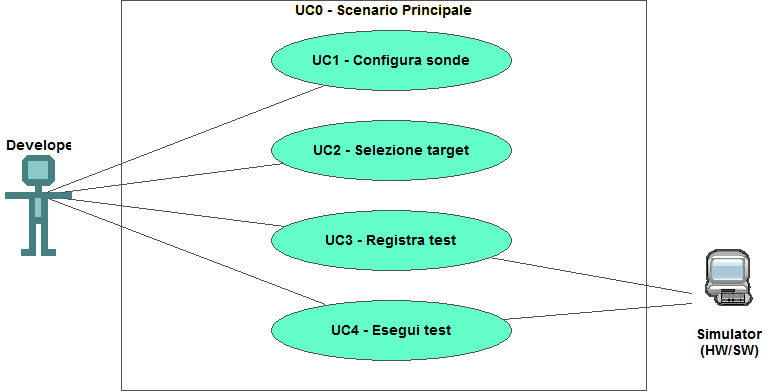
\includegraphics[width=0.9\columnwidth]{usecase/scenario-principale} 
    \caption{Use Case - UC0: Scenario principale}
\end{figure}

\begin{usecase}{0}{Scenario principale}
\usecaseactors{Sviluppatore applicativi}
\usecasepre{Lo sviluppatore è entrato nel plug-in di simulazione all'interno dell'IDE}
\usecasedesc{La finestra di simulazione mette a disposizione i comandi per configurare, registrare o eseguire un test}
\usecasepost{Il sistema è pronto per permettere una nuova interazione}
\label{uc:scenario-principale}
\end{usecase}

\section{Tracciamento dei requisiti}

Da un'attenta analisi dei requisiti e degli use case effettuata sul progetto è stata stilata la tabella che traccia i requisiti in rapporto agli use case.\\
Sono stati individuati diversi tipi di requisiti e si è quindi fatto utilizzo di un codice identificativo per distinguerli.\\
Il codice dei requisiti è così strutturato R(F/Q/V)(N/D/O) dove:
\begin{enumerate}
	\item[R =] requisito
    \item[F =] funzionale
    \item[Q =] qualitativo
    \item[V =] di vincolo
    \item[N =] obbligatorio (necessario)
    \item[D =] desiderabile
    \item[Z =] opzionale
\end{enumerate}
Nelle tabelle \ref{tab:requisiti-funzionali}, \ref{tab:requisiti-qualitativi} e \ref{tab:requisiti-vincolo} sono riassunti i requisiti e il loro tracciamento con gli use case delineati in fase di analisi.

\newpage

\begin{table}%
\caption{Tabella del tracciamento dei requisti funzionali}
\label{tab:requisiti-funzionali}
\begin{tabularx}{\textwidth}{lXl}
\hline\hline
\textbf{Requisito} & \textbf{Descrizione} & \textbf{Use Case}\\
\hline
RFN-1     & L'interfaccia permette di configurare il tipo di sonde del test & UC1 \\
\hline
\end{tabularx}
\end{table}%

\begin{table}%
\caption{Tabella del tracciamento dei requisiti qualitativi}
\label{tab:requisiti-qualitativi}
\begin{tabularx}{\textwidth}{lXl}
\hline\hline
\textbf{Requisito} & \textbf{Descrizione} & \textbf{Use Case}\\
\hline
RQD-1    & Le prestazioni del simulatore hardware deve garantire la giusta esecuzione dei test e non la generazione di falsi negativi & - \\
\hline
\end{tabularx}
\end{table}%

\begin{table}%
\caption{Tabella del tracciamento dei requisiti di vincolo}
\label{tab:requisiti-vincolo}
\begin{tabularx}{\textwidth}{lXl}
\hline\hline
\textbf{Requisito} & \textbf{Descrizione} & \textbf{Use Case}\\
\hline
RVO-1    & La libreria per l'esecuzione dei test automatici deve essere riutilizzabile & - \\
\hline
\end{tabularx}
\end{table}%             %Analisi dei requisiti
\chapter{Recupero dell'informazione}
\label{cap:recupero-informazione}
Perché, quando consultiamo un libro in biblioteca, capita che ci venga richiesto di non ricollocarlo nello scaffale e bensì di lasciarlo sul tavolo(o su un apposito carrello)? Perché un libro collocato nel posto sbagliato è un libro "perso": se si trova nella posizione errata è molto più difficile da reperire. Lo stesso vale per qualsiasi informazione: non importa solo possederla, importa anche se riusciamo a recuperarla.
Abbiamo quotidianamente bisogno di recuperare informazioni: non è strano quindi che sia un ambito di studio da ben prima che nascessero i calcolatori.\footnote{si veda, per esempio \url{https://en.wikipedia.org/wiki/Bible_concordance}} I metodi che possiamo utilizzare dipendono sia dalla potenza di calcolo che dalla quantità di dati che abbiamo a disposizione: finché i dati sono pochi, il miglior classificatore rimane comunque quello umano. (non a caso esistono progetti di crowdsourcing come \gls{Amazon-Mechanical-Turk})

Possibili esempi di recupero dell'informazione potrebbero essere il trovare: 
\begin{itemize}
\item motivetto musicale che abbiamo in testa;
\item un quadro di cui non ricordiamo nome e/o autore;
\item se esiste una libreria o un framework che faccia il caso nostro;
\item le foto che abbiamo fatto qualche anno prima a un bel paesaggio;
\item un paper di cui avremmo bisogno, ma non sappiamo se effettivamente esiste.
\end{itemize}

È chiaro quindi che quello che noi vogliamo reperire non è sempre di natura testuale (nel caso dello stage, infatti, si tratta di video) e il modo in cui noi andremo interagire con il nostro sistema informativo non si limita a esprimere una query testuale: ci sono però alcuni elementi base in comune che possiamo individuare.

\section{Esigenza informativa, interrogazione e risultati}
Per interrogare un sistema di recupero dell'informazione, dobbiamo esprimere la nostra esigenza informativa con una query: il sistema quindi ritornerà i documenti che ritiene siano rilevanti rispetto alla nostra richiesta. Sia l'interrogazione che documenti, come già visto in precedenza, non sono necessariamente in formato testuale. Un risultato è considerato pertinente quando risponde al nostro bisogno informativo: questo in concreto significa che, per esempio, se stiamo facendo una ricerca all’interno di un corpus testuale, non stiamo semplicemente cercando di ottenere i documenti in cui un termine compare (quindi un pattern match su una stringa): questo è da tenere a mente quando si va a valutare un sistema di IR.

\section{Indicizzazione}
Per compiere una ricerca all’interno di un corpus abbiamo bisogno di un indice con cui compiere la ricerca desiderata, indipendentemente che si tratti di una ricerca sui metadati o full-text. Nel caso di una ricerca full-text, in particolare, abbiamo bisogno di una fase di analisi lessicale del nostro testo per ridurlo in unità più semplici, ovvero i \gls{token}. Le scelte che noi compiamo nella creazione dell'indice influenzano anche cosa noi saremo in grado di ritornare e quindi bisogna risolvere problematiche del tipo:

\begin{itemize}
    \item come tokenizzare i documenti ("Sant’Angelo” è un token solo o sono due?);
    \item quali token sono presenti nel mio corpus e in quali documenti;
    \item come tokenizzare i documenti.
\end{itemize}


Sebbene non fosse obiettivo dello stage quello di migliorare l’indicizzazione, si è rivelato indispensabile capire sia come costruirlo che come poterlo modificare.

\subsection{Come memorizzare i token}
Oltre a ridurre i nostri documenti in token, abbiamo bisogno di trovare un modo per memorizzarli: riuscire a stabilire in quali documenti è presente un token è utile per capire quali documenti potremmo voler ritornare all’utente. Abbiamo quindi bisogno di:
\begin{itemize}
    \item conoscere i token disponibili nel corpus;
    \item dato un token, scoprire in quali documenti è presente.
\end{itemize}

Stabilire velocemente la presenza o meno di un token in un corpus è utile per avere buoni tempi di risposta della ricerca: nel caso particolare della libreria utilizzata per il recupero dell'informazione, l'insieme dei token disponibili è implementato come una macchina a stati finiti. Questa scelta ha i suoi vantaggi e i suoi svantaggi.
Tra i vantaggi principali:
\begin{itemize}
    \item ridotto footprint della memoria
    \item velocità nello stabilire se un token è presente nel corpus 
\end{itemize}
con il compromesso però di dover avere un indice pensato per essere immutabile (p.es. ha influito nella creazione del tesauro automaticamente generato e relativo indice).

Per scoprire in quali documenti è presente un token, abbiamo bisogno di sapere tre cose:
\begin{itemize}
\item posting list;
\item inverted index.
\end{itemize}

\begin{description}
    \item[posting list]: una lista di indici di documenti. Ogni documento è infatti identificato da un codice univoco. \newline{}
    Esempio: (23, 42, 67, 313)
    \item[inverted index]: set di tuple del tipo \textit{<token, posting list>}. \newline{}
    Esempio: (<'hello', (23, 42, 67, 313)>, <'world', (13, 18)>)
\end{description}

Per stabilire in quali documenti il token è presente, dobbiamo quindi fare uso dell'inverted index.


\subsection{Minificare un indice}
Assumiamo, senza perdere di generalità, che i token siano composti da un solo termine.
Per riuscire a minificare il nostro indice, vorremmo che le declinazioni diverse di uno stesso termine fossero mappate nella stessa tupla del nostro indice inverso (e quindi considerate come un termine unico).

Esempio: "documentai" e "documentavo" dovrebbero essere mappate nello stesso indice inverso, come potrebbe essere il termine "documentare".

Per farlo abbiamo almeno due modi: usare un lemmatizer o usare uno stemmer.

\begin{description}
    \item[Lemma]: la forma di un termine che troviamo in un dizionario. \newline
    Esempio: "documentavo" diventa "documentare"
    \item[Stem]: una forma troncata del termine. \newline
    Esempio: "documentavo" diventa "document"
\end{description}

Riuscire a trovare la forma corretta "da dizionario" è un lavoro complicato da formalizzare; un esempio evidente ci arriva dalla Pagina della Sfinge de "La Settimana Enigmistica": mattino e mattone non sono rispettivamente diminutivo e accrescitivo di matto.

Lo stemmer si propone un obiettivo meno ambizioso, ma che comunque funziona altrettanto bene quando il nostro obiettivo è il recupero dell'informazione.

\newpage

\section{Modelli di recupero dell'informazione}
\begin{center}
\begin{figure}
    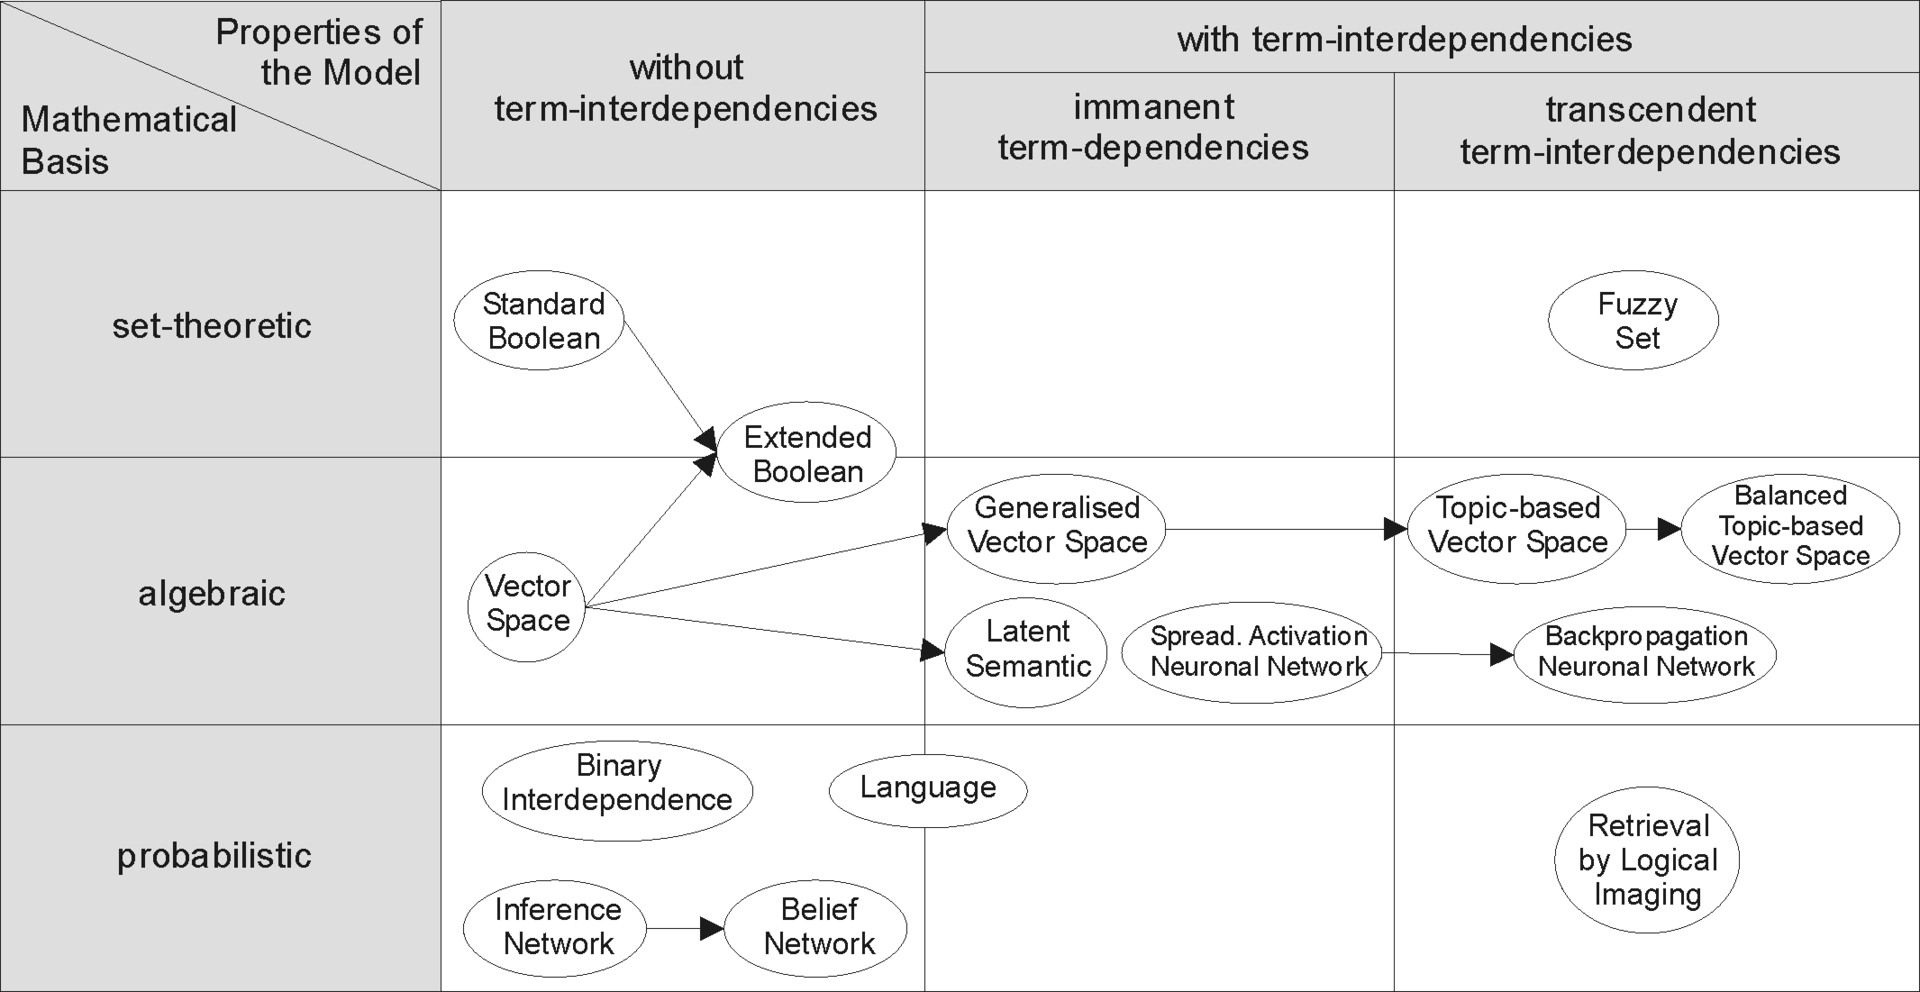
\includegraphics[scale=0.70]{immagini/Information-Retrieval-Models.png}
    \caption{Modelli di recupero dell'informazione}
 \end{figure}
\end{center}
Come rappresentiamo i documenti e interrogazione dipende principalmente del modello di recupero scelto: questo influenza le strategie di recupero e, inevitabilmente, la rappresentazione più conveniente.

Possiamo categorizzare i modelli di recupero in base a:
\begin{itemize}
    \item se viene o meno rappresentata l'interdipendenza tra i termini;
    \item classificazione matematica.
\end{itemize}

Per quanto riguarda lo stage, ci si è limitati ai modelli algebrici: in particolare al modello a spazio vettoriale e al latent semantic indexing.


\subsection{Bag of words}
È un modello di rappresentazione dei documenti che ignora l'ordine dei termini: per ogni termine in un documento, si considera la tupla \textit{<termine, \#occorrenze nel documento>}. 

\subsection{Modello a spazio vettoriale}
Il modello a spazio vettoriale consiste nel rappresentare i documenti e le interrogazioni come dei vettori in uno spazio $|V|$-dimensionale, dove $|V|$ è pari al numero di termini: si tratta, tipicamente di vettori molto sparsi.

\subsection{Definire la distanza tra due documenti}
Per definire la distanza tra due documenti $d$ e $q$ nello spazio vettoriale (o documento e una interrogazione), un'idea potrebbe essere quella di calcolare la loro distanza euclidea.
\begin{equation}
    dist(\mathbf{d},\mathbf{q}) = \sqrt{\sum_{i=1}^n {(d_i-q_i)^2}}    
\end{equation}

Assumiamo che $q$ sia uguale al documento $d$ più il documento $d$ stesso appeso alla fine (quindi due volte $d$): dal punto di vista semantico sono identici, ma la distanza tra i due può essere piuttosto grande e quindi la distanza euclidea è inadatta per misurare la similarità tra due documenti.

Pensando alla rappresentazione a spazio vettoriale, è evidente che $d$ e $q$ manterrebbero comunque lo stesso angolo rispetto l'origine: per valutare la similarità conviene quindi considerare l'angolo, o meglio ancora il coseno, invece che la distanza euclidea.
\begin{equation}
\text{similarità} = \cos(\theta) = {\mathbf{d} \cdot \mathbf{q} \over \|\mathbf{d}\| \|\mathbf{q}\|} = \frac{ \sum\limits_{i=1}^{n}{d_i  q_i} }{ \sqrt{\sum\limits_{i=1}^{n}{d_i^2}}  \sqrt{\sum\limits_{i=1}^{n}{q_i^2}}}
\end{equation}

Questo perché, più due documenti sono simili e più è piccolo l'angolo che li separa, mentre noi vorremmo assegnare un valore più alto all'aumentare della similarità (cosa che succede con il coseno). 

\section{Scoring}
Per misurare l'importanza di un termine rispetto a un documento, vorremmo tenere conto di due fattori:
\begin{itemize}
    \item quante volte il termine compare nel documento (\textbf{term frequency});
    \item l'informatività del termine (\textbf{inverse document frequency}).
\end{itemize}

\subsection{Term frequency}
Rappresenta quante volte il termine compare nel documento:
\begin{equation}
    tf_{t,d} = 1 + log_2(\text{\#occorrenze del termine t nel documento d})
\end{equation}

La rilevanza di un termine non cresce in maniera lineare con l'aumentare del numero delle occorrenze: per questo ci interessa il logaritmo e non il numero delle occorrenze.

\subsection{Inverse document frequency}
Rappresenta l'informatività di un termine:
\begin{equation}
    idf_t = log_2(\frac{\text{\#documenti del corpus}}{\text{\#documenti che contengono il termine t}})
\end{equation}

Un termine raro ci dice molto di più su un documento che uno frequente\footnote{Si veda il concetto di entropia nella teoria dell'informazione: \url{https://en.wikipedia.org/wiki/Entropy_(information_theory)}}; anche in questo caso il logaritmo ci serve per ridurre il valore finale (nei casi in cui il numero dei documenti è elevato).

\subsection{tf-idf}
Si definisce tf-idf di un documento d e un termine d come:
    \begin{equation}
        tf\-idf_{t,d} = tf_{t,f} * idf_{t}
    \end{equation} 

ovvero l'unione tra il numero di occorrenze di un termine in un documento e l'informatività del termine nel documento.

$tf\-idf_{t,d}$ assegna un peso nel documento d che è:
\begin{itemize}
    \item il più alto, quando t compare molte volte in un piccolo numero di documenti;
    \item più basso, quando un termine compare poche volte oppure in molti documenti;
    \item minimo, quando un termine compare praticamente tutti i documenti.
\end{itemize}

\subsection{Matrice termini-documenti}
La nostra collezione di N documenti può essere vista, oltre che come una collezione di N vettori, come una matrice termini-documenti: una matrice le cui righe rappresentano i termini e le colonne i documenti.


\section{Ranking}
Una volta stabilito quali documenti devono vogliamo ritornare da una ricerca, dobbiamo capire come possiamo ordinare i risultati: non tutti i risultati meritano la stessa attenzione da parte dell'utente, che di norma non andrà a controllarli tutti.

Nel caso specifico del progetto, si utilizza Okapi BM25 per lo scoring dei documenti,
Data una interrogazione $Q$, con $q_1, \dots , q_n$ parole chiave, il BM25 score è 

\begin{equation}
    \text{score}(D,Q) = \sum_{i=1}^{n} \text{IDF}(q_i) \cdot \frac{\text{(\#occorrenze di q\textsubscript{i} in D)} \cdot (k_1 + 1)}{\text{(\#occorrenze di q\textsubscript{i} in D)} + k_1 \cdot \left(1 - b + b \cdot \frac{|D|}{\text{avgdl}}\right)}
\end{equation}

dove $|D|$ è il numero di termini nel documenti D, $avgdl$ è lunghezza media dei documenti del corpus, $k_1$ e $b$ parametri liberi.

\section{Tollerant retrieval}
Ammettere una certa tolleranza nel recupero dell’informazione può essere d’aiuto per aumentare la recall (prestando ovviamente attenzione a non peggiorare troppo la precision). Nel caso specifico del progetto, una tipologia d'errore era quella delle parole che suonavano in maniera simile: per esempio "SitePainter" veniva trascritto "serpente".

L’uso di \gls{algoritmi-fonetici} come Soundex, Metaphone e Double Metaphone purtroppo si è rivelato essere inefficace per correggere questi errori. Esiste anche una versione più aggiornata di Metaphone (la 3), ma per motivi di licenza\footnote{Nonostante esista una versione open-source rilasciata con licenza BSD, l'autore della libreria non ne permette il porting in altri linguaggi \url{https://github.com/threedaymonk/text/issues/21\#issuecomment-67752327}} si è preferito non tentare questa strada.

\subsection{Stopwords}
Filtrare le stopword ci può essere d’aiuto nel migliorare la precisione, ma determinare cosa togliere e cosa no non è banale. Un possibile approccio potrebbe essere quello di escludere quei termini che sono uniformemente distribuiti nel corpus (come gli articoli, i pronomi, le preposizioni, le congiunzioni e le interiezioni), ma anche così si rischia di eliminare informazioni solo all'apparenza ininfluenti: esempio classico inglese è "to be or not to be".

\section{Valutazione di un sistema di recupero dell'informazione}
Per riuscire a migliorare il nostro sistema, dobbiamo prima capire come possiamo misurare (e gli eventuali limiti delle misure)

Il nostro sistema ideale dovrebbe:
\begin{itemize}
    \item ritornare tutti i risultati pertinenti;
    \item i risultati ritornati dovrebbero essere tutti pertinenti.
\end{itemize}

Purtroppo l’ideale si scontra con l’ideale e dobbiamo trovare un compromesso tra le due proprietà desiderate: quindi ci interessa capire quanto in sistema di \gls{ir} soddisfa queste due proprietà e a tale scopo definiremo la precision e la recall.


\subsection{Vero positivo, falso positivo, vero negativo, falso negativo}
\begin{center}
    \begin{figure}
        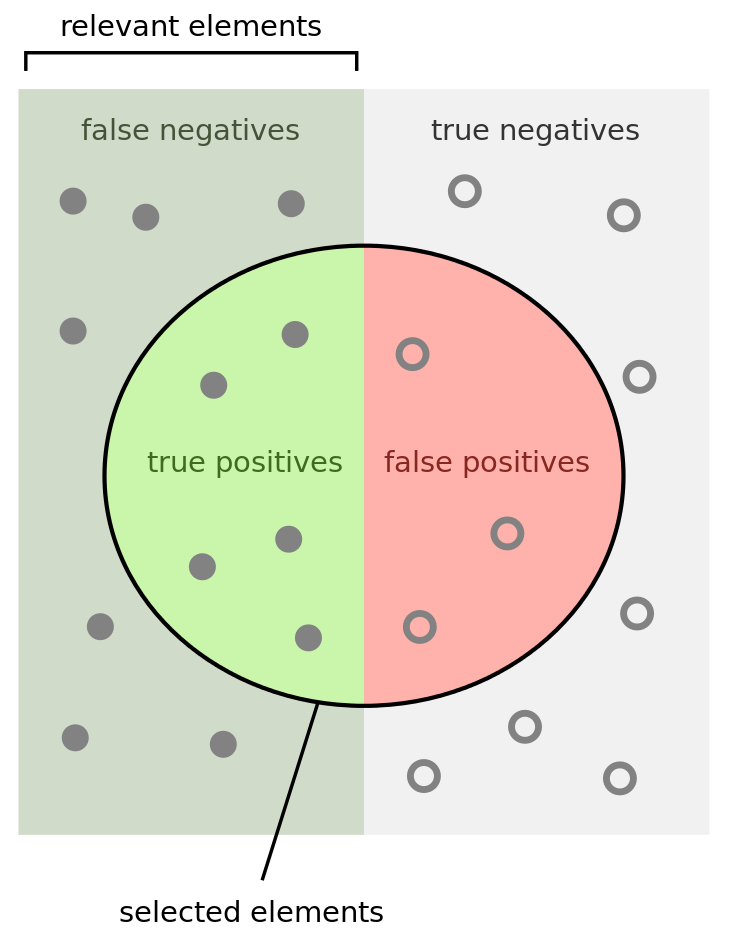
\includegraphics[scale=0.2]{immagini/truefalsenegativepositive.png}
        \caption{Veri/falsi positivi e veri/falsi negativi}
    \end{figure}
\end{center}
Data una interrogazione $q$ e un documento $d$, il risultato dell'interrogazione è un:
\begin{itemize}
    \item \textbf{falso positivo} se il documento $d$ non è rilevante per la ricerca, ma è stato ritornato;
    \item \textbf{vero positivo} se il documento $d$ è rilevante per la ricerca ed è stato ritornato;
    \item \textbf{falso negativo} se il documento $d$ è rilevante per la ricerca, ma non è stato ritornato;
    \item \textbf{vero negativo} se il documento $d$ non è rilevante per la ricerca, e non è stato ritornato;
\end{itemize}

\FloatBarrier

\subsection{Metriche di valutazione}
\label{sub:metriche-valutazione}
\begin{center}
\begin{figure}
    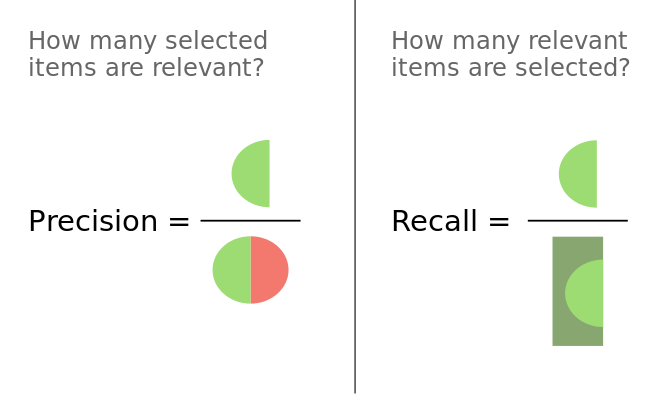
\includegraphics[scale=0.2]{immagini/precisionrecall.png}
    \caption{Precisione e recall}
\end{figure}
\end{center}
\begin{description}
    \item[recall] di una interrogazione a un sistema IR è definita come:
    \begin{equation}
        \mbox{Precisione}=\frac{|\{\mbox{documenti attinenti}\}\cap\{\mbox{documenti recuperati}\}|}{|\{\mbox{documenti recuperati}\}|}
    \end{equation}
    ovvero ci da una misura di quanti dei risultati pertinenti presenti nel corpus siamo riusciti a recuperare e quindi dei falsi negativi di una interrogazione. 
    \item[precision] di una interrogazione a un sistema IR come: 
    \begin{equation}
        \mbox{Recupero}=\frac{|\{\mbox{documenti attinenti}\}\cap\{\mbox{documenti recuperati}\}|}{|\{\mbox{documenti attinenti}\}|} 
    \end{equation}
    ovvero ci da una misura della bontà dei risultati recuperati e quindi della quantità di falsi positivi.
\end{description}
Ambedue sono facilmente riformulabili in termini di vero positivo, falso positivo, vero negativo e falso negativo. Nel decidere a quale delle due dare la priorità, bisogna tenere conto dei due estremi:
\begin{itemize}
    \item per avere una recall pari a 1, è sufficiente ritornare tutti i documenti;
    \item nel cercare di avere una precision tendente a 1, c'è il rischio di essere eccessivamente selettivi. 
\end{itemize}

\begin{description}
    \item[f-measure] Abbiamo quindi bisogno di un buon bilanciamento tra recall e precision. Una misura che sintetizzi le due precedenti è chiamata f-measure e corrisponde alla media armonica tra precision e recall. 
    \begin{equation}
        F_1 = 2 \cdot \frac{\mathrm{precision} \cdot \mathrm{recall}}{\mathrm{precision} + \mathrm{recall}}
    \end{equation}
    
    Calcolare la media aritmetica tra precision e recall sarebbe ancora più facile, ma tale valore sarebbe poco significativo per valutare la bontà della nostra ricerca. (i.e. si potrebbe ritornare sempre l'intero corpus e ottenere sempre una media aritmetica di 0.5)
\end{description}


\FloatBarrier

\subsection{Gold standard} 
Per valutare un sistema di reperimento dell’informazione non è sufficiente valutare come si comporta con rispetto a una interrogazione, ma rispetto a un numero congruo di interrogazioni.
Come rule of thumb, 50 interrogazioni sono considerate un numero congruo, anche se bisogna considerare altri vincoli che cambiano le carte in tavola( nel caso particolare del progetto, era richiesto che le query dovessero contenere falsi positivi, oltre al solito vincolo di avere un corpus piccolo).

Per ogni interrogazione, bisogna quindi segnare quali documenti sono pertinenti (dove, con pertinente, si considera sempre il soddisfacimento o meno del bisogno informativo dell’utente): è il cosiddetto \gls{gold-standard} o ground truth.

Con queste informazioni, è quindi possibile (e facile) calcolare precision, recall e f-measure per ogni interrogazione: purtroppo la costruzione di una gold standard richiede anche parecchio tempo.          % Introduzione al recupero dell'informazione
\chapter{Latent Semantic Indexing}
\label{cap:latent-semantic-indexing}
Prendiamo come esempio la seguente matrice termini-documenti:
\begin{equation*}
    \mathbf{A}=
    \begin{blockarray}{*{6}{c} l}
      \begin{block}{*{6}{>{$\footnotesize}c<{$}} l}
        $D_1$ & $D_2$ & $D_3$ & $D_4$ & $D_5$ & $D_6$ & \\
      \end{block}
      \begin{block}{[*{6}{c}]>{$\footnotesize}l<{$}}
        1 & 1 & \textbf{\underline{0}} & 1 & 0 & 0 \bigstrut[t]& internet \\
        1 & \textbf{\underline{0}} & 1 & 1 & 0 & 0 & web \\
        1 & 1 & 1 & 2 & 1 & 1 & surfing \\
        0 & 0 & 0 & 1 & 1 & 1 & beach \\
      \end{block}
    \end{blockarray}
  \end{equation*}

È evidente che i concetti della collezione sono 2: uno riguarda il mondo dell'informatica(web) e l'altro dello sport(surf): in questo caso internet e web sono sinonimi, mentre surf può avere più significati. Assumiamo quindi che i primi 4 documenti si riferiscano al mondo dell'informatica, mentre i primi due invece a quello dello sport. Vorremmo quindi che il termine web e il termine internet fossero considerati come presenti anche nei documenti $D_2$ e $D_3$ e passare quindi da $A$ alla matrice modificata $A'$:

  \begin{equation*}
    \mathbf{A'}=
    \begin{blockarray}{*{6}{c} l}
      \begin{block}{*{6}{>{$\footnotesize}c<{$}} l}
        $D_1$ & $D_2$ & $D_3$ & $D_4$ & $D_5$ & $D_6$ & \\
      \end{block}
      \begin{block}{[*{6}{c}]>{$\footnotesize}l<{$}}
        1 & 1 & \textbf{\underline{1}} & 1 & 0 & 0 \bigstrut[t]& internet \\
        1 & \textbf{\underline{1}} & 1 & 1 & 0 & 0 & web \\
        1 & 1 & 1 & 2 & 1 & 1 & surfing \\
        0 & 0 & 0 & 1 & 1 & 1 & beach \\
      \end{block}
    \end{blockarray}
  \end{equation*}

  In questo modo è possibile recuperare, per esempio, il documento $D_2$ anche cercando "web".
  Notiamo anche che il rango della matrice modificata è 2, mentre il rango della matrice originale è 4.
  Una base di $A'$ è infatti:
  \begin{equation}
    \mathbf{B} = \begin{pmatrix}
        1 & 0 \\
        1 & 0 \\
        1 & 1 \\
        0 & 1 \\   
    \end{pmatrix}
\end{equation}

La base $B$ è la matrice che rappresenta i concetti della matrice originale, mentre $D$ è la rappresentazione dei documenti nello spazio dei concetti, dove $A = B \cdot D$
Nel caso particolare, D vale quindi:

 \begin{equation*}
    \mathbf{D}=
    \begin{blockarray}{*{6}{c} l}
      \begin{block}{*{6}{>{$\footnotesize}c<{$}} l}
        $B_1$ & $B_1$ & $B_1$ & $B_1 + B_2$ & $B_1$ & $B_1$ \\
      \end{block}
      \begin{block}{[*{6}{c}]>{$\footnotesize}l<{$}}
        1 & 1 & 1 & 1 & 0 & 0 \\
        0 & 0 & 0 & 1 & 1 & 1 \\
      \end{block}
    \end{blockarray}
  \end{equation*}

\section{Obiettivo della LSI}
Dati $A$, $k$ tali che: 
\begin{itemize}
    \item  $A$: matrice termini documenti di dimensione $mxn$
    \item  $k <  rango(A)$
\end{itemize}
trovare $A'$ di rango $k$ tale che la differenza tra $A'$ e $A$ sia la più piccola possibile.

\begin{equation*}
 \mathbf{A'} = argmin_{A'_{m x n} \text{con rango k}} \norm{A - A'}
\end{equation*}

\section{Calcolare A'}
\begin{theorem}
Data una matrice A qualsiasi di dimensione $m x n$ e rango $k$, esistono $U$, $S$, $V$ tali che $A = U \cdot S \cdot V$ , dove:
\begin{itemize}
    \item $U$ è una matrice $m \cdot k$ con $U^T \cdot U = I_k$
    \item $S$ è una matrice diagonale $k \cdot k$
    \item $V$ è una matrice $k \cdot k$ con $V \cdot V^T = I_k$
\end{itemize}
\end{theorem}
Tale decomposizione è detta decomposizione ai valori singolari o SVD. Utilizzando la decomposizione ai valori singolari è quindi possibile calcolare il valore di $A$.

\noindent Posto $A = U \cdot S \cdot V$ la SVD di A:
\begin{itemize}
    \item $U_k$ = le prime $k$ colonne di $U$
    \item $S_k$ = la parte superiore $k \cdot k$ di $S$
    \item $V_k$ = le prime $k$ righe di $V$
\end{itemize}

e $A_k = U_k *  V_k * U_k$, allora $A' = A_k$, ovvero la matrice che minimizza $\norm{A - A'}$.

\section{Calcolare la SVD}
Il calcolo della decomposizione ai valori singolari si basa su una generalizzazione della \gls{edv}. La matrice $A$ termini-documenti è, infatti, una matrice rettangolare, mentre una precondizione per poter applicare la decomposizione agli autovettori è quella di avere una matrice quadrata.
Per quanto riguarda la libreria scelta per il calcolo della decomposizione, l'algoritmo attualmente implementato è quello di Golub-Kahan.\footnote{Questo emerge esaminando la libreria \url{https://github.com/lauerfab/MLweb/blob/92142d92abd64b12b251a43966d354328e3c9bbb/lalolab/src/linalg.js\#L6844}}

L'algoritmo di Golub-Kahan calcola la \gls{svd} in due passi:
\begin{enumerate}
    \item riduce la matrice a una matrice bidiagonale utilizzando una sequenza di trasformazioni di Householder;
    \item riduce la superdiagonale della matrice, utilizzando una sequenza di trasformazioni di Givens.
\end{enumerate} 

\section{Migliorare la ricerca utilizzando la LSI}
Per migliorare la ricerca utilizzando la \gls{lsi}, ci sono almeno 3 possibilità:
\begin{enumerate}
    \item utilizzare la matrice $A_k$ al posto della matrice $A$
    \item utilizzare la matrice $V_k$ al posto della matrice $A$
    \item espandere la matrice originale $A$.
\end{enumerate} % Introduzione all'analisi della semantica latente
% !TEX encoding = UTF-8
% !TEX TS-program = pdflatex
% !TEX root = ../tesi.tex

%**************************************************************
\chapter{Progettazione e sviluppo}
\label{cap:progettazione-sviluppo}
%**************************************************************

\intro{Il capitolo approfondisce come si è affrontato il problema, le tecnologie e le scelte fatte nel progetto.}\\

\section{Procedura di lavoro}
Il tutor aziendale si è sempre dimostrato molto disponibile durante tutta la durata dello stage. Non sono stati usati sistemi di ticketing per segnalare lo stato di avanzamento del lavoro, ma si è lavorato in maniera più informale e diretta. 

Le proposte di miglioramento (p.es. \gls{algoritmi-fonetici}) e  su come implementare (p.es. ricerche aggregate), sono state prima raccolte in un foglio su Google Doc e poi discusse di persona con il tutor.

\subsection{Individuazione del materiale}
Parte del lavoro è stata riuscire a reperire del materiale di studio adatto: tale ricerca è iniziata una settimana circa prima dell'inizio effettivo dello stage. Il materiale inizialmente ricercato riguardava la parte di:
\begin{itemize}
    \item recupero dell'informazione
    \item Javascript
\end{itemize}
sia cartaceo, che elettronico, disponibile grazie all'ateneo\footnote{\url{https://catalogo.unipd.it}}. 

\subsection{Realizzazione di un prototipo}
Dopo infarinatura iniziale degli argomenti principali di recupero dell'informazione e uno studio della libreria lunr.js, si è proceduto quindi con la realizzazione di un primo prototipo di ricerca, che consentisse la ricerca all'interno del \gls{corpus}(che sono stati convertiti in \gls{json}\glsfirstoccur{} utilizzando NodeJS). 
Al prototipo iniziale, è stato quindi aggiunto uno stemmer italiano e delle stopword: il prototipo così ottenuto è stata la base di confronto rispetto alle versioni successive (ovvero quelle che implementano l'uso di tesauri e l'analisi della semantica latente). 

\subsection{Tesauro generato manualmente}
Quindi si è passati alla realizzazione manuale di un tesauro: molto semplice dal punto di vista della programmazione (si tratta di una PipelineFunction\footnote{\url{https://lunrjs.com/docs/lunr.PipelineFunction.html}} di lunr.js che espande le interrogazioni con i sinonimi dei termini richiesti dall'utente), più difficile ed oneroso in termini di tempo dal punto di vista della compilazione del tesauro.
La strategia adottata inizialmente è stata lo studio delle frequenze dei termini e degli stem, che però si è rivelata essere infruttuosa; la strategia adottata alla fine è stata, su proposta del candidato, quella di utilizzare il modello di \gls{pos-tagger}\glsfirstoccur{} allenato da un altro tesista.

\subsection{Piano di test}
Si è allora passati alla creazione di un piano di test: tale attività sarebbe dovuta avvenire a monte della soluzione basata su tesauro costruito manualmente ma così non è stato, per la difficoltà rivelatasi nell'individuare delle interrogazioni con falsi negativi; questa inversione se non altro ha garantito che i dati del tesauro non fossero appositamente costruiti in base ai test pianificati. 

\subsection{Tesauro generato automaticamente}
La realizzazione di un tesauro automaticamente generato ha richiesto un'ulteriore approfondimento studio: sia per quanto riguarda il recupero dell'informazione che per, nello specifico, la generazione automatica di un tesauro (sia su libri di testo che su paper). La scelta di utilizzare co-occorrenze nella costruzione dei sinonimi è stata dettata dalla limitazione della dimensione del tesauro stesso:

\begin{center}
    "\textit{synonyms do not cooccur, but rather have similar cooccurrence patterns}"
\end{center}

Il tesauro così composto individua bene le parole composte (utile per la migliorare la precisione) e non i sinonimi. 

\subsection{Refactoring e tesauro generico}
Prima di integrare un tesauro generico si è proceduto a:
\begin{itemize}
    \item refactoring del codice;
    \item conversione del tesauro di LibreOffice con l'utilizzo della libreria thesaurus.
\end{itemize}

\subsection{Analisi della semantica latente}
Per poter implementare la soluzione dell'analisi della semantica latente, è stato necessario:
\begin{itemize}
    \item individuare ulteriore materiale di studio;
    \item individuare una libreria per il calcolo della \gls{svd};
    \item approfondire lo studio della libreria lunr.js.
\end{itemize}

Per quanto riguarda la parte teorica, è stato di fondamentale aiuto il tutor aziendale; per riuscire poi a implementarlo è stato necessario un approfondimento su come viene implementata la ricerca da lunr.js(leggendo il codice della libreria).

\subsection{Documentazione}
Infine, è stata realizzata la documentazione del codice, utilizzando \gls{jsdoc}.
%**************************************************************
\section{Librerie}
Fatta eccezione per lunr.js, le librerie scelte sono state proposte dal candidato; il vincolo principale era, per le librerie che avrebbero dovuto permettere la ricerca, di essere scritte in Javascript (preferibilmente eseguibili lato browser).
Nella scelta delle librerie i dei linguaggi, si è tenuto conto dei seguenti criteri:
\begin{itemize}
    \item possibilità di essere eseguita via browser;
    \item funzionalità disponibili;
    \item dipendenze;
    \item supporto e sviluppo;
    \item disponibilità di documentazione.
\end{itemize}

\subsection{Lunr.js}
%\begin{figure}
%    
\includegraphics[scale=0.15]{immagini/lunrjs-logo.jpg}
%    \caption{Logo di Lunr.js}
% \end{figure}
lunr.js è una libreria semplice da utilizzare, ma comunque potente: permette di fornire la funzionalità ricerca senza aver necessariamente bisogno di servizi esterni. 
È pensata per essere utilizzata con collezioni relativamente piccole: ciò nonostante, non trascura l'aspetto dell'efficienza (sia il costo computazionale delle operazione che lo spazio occupato in memoria). 
Non ha dipendenze esterne e può essere eseguita sia da browser che all'interno di un server Node.js.
È stata utilizzata per l'indicizzazione e per la ricerca dei documenti all'interno del \gls{corpus}.

\FloatBarrier

\subsection{LALOLib}
LALOLib (Linear ALgebra Online Library) è una libreria interamente scritta in Javascript: rende facile effettuare operazioni algebriche direttamente da browser. È eseguibile sia in modalità sincrona che asincrona. È sviluppata dal Laboratoire Lorrain de Recherche en Informatique et ses Applications come parte del progetto MLweb costituisce il core di LALOLab (un ambiente di calcolo scientifico online). È anche alla base di ML.js, una libreria in Javascript library per il machine learning. 
LALOLib include funzioni per:
\begin{itemize}
    \item algebra lineare;
    \item statistica;
    \item ottimizzazione (con glpk.js);
    \item machine learning (con ML.js).
\end{itemize}

La scelta della libreria è stata vincolata, a causa della scarsità di librerie di calcolo scientifico in Javascript che siano al contempo attivamente sviluppate e che supportino il calcolo della \gls{svd} (p.es. tensorflow.js\footnote{\url{https://github.com/tensorflow/tfjs/issues/110}} allo stato attuale non lo permette e sushi2\footnote{\url{https://github.com/mil-tokyo/sushi2}} non è più sviluppata da quasi 3 anni) 

È stata utilizzata per effettuare i calcoli matriciali necessari allo sviluppo del tesauro automaticamente generato(i.e. il calcolo della matrice delle similarità) e per l'analisi della semantica latente.


\subsection{NumPy}
NumPy è una libreria open source per il linguaggio di programmazione Python, che aggiunge supporto a grandi matrici e array multidimensionali insieme a una vasta collezione di funzioni matematiche di alto livello per poter operare efficientemente su queste strutture dati. È stato creato nel 2005 da Travis Oliphant basandosi su Numeric di Jim Hugunin. È stato utilizzato come confronto delle performance della libreria LALOLib nel calcolo della decomposizione ai valori singolari della matrice termini-documenti normalizzata (necessario per l'analisi della semantica latente). In particolare, fa uso della routine \texttt{\_gesdd} della libreria LAPACK (scritta in Fortran) per il calcolo della \gls{svd}; è stata scelta questa libreria e non SciPy come termine di confronto in quanto entrambe non sfruttano la sparsità della matrice nel calcolo della \gls{svd}.

\subsection{scikit-learn}
Scikit-learn è una libreria open source di apprendimento automatico per il linguaggio di programmazione Python, progettata per operare con le librerie NumPy e SciPy: è stata scelta dal candidato per prendere familiarità inizialmente con il dominio (recupero dell'informazione).

\subsection{OpenNLP}
Apache OpenNLP è una libreria per l'elaborazione del linguaggio naturale facendo uso del machine learning.
Supporta, per esempio, il riconoscimento del linguaggio, tokenization, POS tagging, chunking e molto altro. È stata utilizzata per il POS tagging, utilizzando un modello allenato da un altro tesista\footnote{Jiancheng Ye, laureando in Ingegneria Informatica presso l'Università degli Studi di Padova}.

\subsection{Riepilogo}
 Un riepilogo delle librerie utilizzate, per linguaggio e scopo.
 \begin{center}
    \begin{tabular}{p{0.15\linewidth}lp{0.5\linewidth}}
        \toprule
        Linguaggio & Libreria & Scopo \\
        \midrule
          Javascript (browser) & lunr.js & Indicizzare i documenti, filtrare alcuni termini irrilevanti al fine delle ricerche tramite stopword, configurare uno stemmer, effettuare le ricerche sull'indice creato e quindi ritornare i documenti recuperati in base al loro score. \\
           & LALOLib & Effettuare i calcoli matriciali necessari per la generazione automatica di un tesauro (i.e. calcolo della matrice delle similarità) e per l'analisi della semantica latente (i.e. \gls{svd}, moltiplicazioni tra matrici) \\
           \addlinespace
          NodeJS &  srt-to-json & Convertire i file delle trascrizioni in un JSON rappresentante il \gls{corpus} dei documenti. \\
                 &  thesaurus & Convertire il tesauro generico di LibreOffice in JSON, per permettere il suo utilizzo all'interno del progetto.\\
        \addlinespace
          Python & NumPy        & Confronto delle performance del calcolo della decomposizione ai valori singolari \\
                 & scikit-learn & Studio iniziale del recupero dell'informazione.\\
        \addlinespace
          Java   & OpenNLP      & Taggare i termini in base alla parte del discorso. (per il tesauro generato manualmente)\\
        \bottomrule
    \end{tabular}
        \captionof{table}[Riepilogo librerie]{Librerie utilizzate durante lo stage} 
        \label{tab:librerieUsate}
    \end{center}
\newpage
\section{Indicizzazione}
\begin{figure}
    \centering
    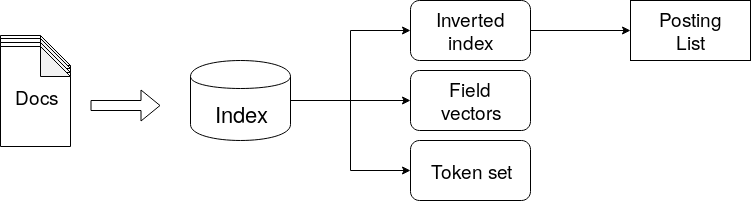
\includegraphics[scale=0.42]{immagini/indice.png}
    \caption{Indice}
    \label{fig:indice}
\end{figure}
    
La struttura dell'indice rispecchia quella impostata dalla libreria lunrjs. L'indice è dotato quindi di:
\begin{itemize}
    \item inverted index, che permette di conoscere la posting list per ogni token;
    \item field vectors, ovvero la rappresentazione interna dei documenti (come sparse vector);
    \item token set, i token presenti nei documenti, rappresentati come una macchina a stati finiti.
\end{itemize}
 
I calcoli matriciali, necessari per la generazione automatica del tesauro e per l'analisi della semantica latente, utilizzano la libreria LALOLib e non sfruttano la sparsità. (perché non si sono trovate libreria in Javascript che calcolino la \gls{svd} e sfruttino la sparsità) 

%*************************************************************
\begin{figure}
    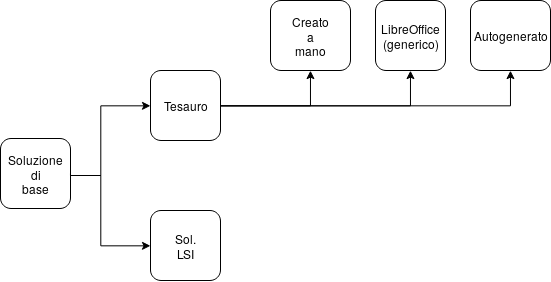
\includegraphics[scale=0.6]{immagini/schema-soluzione.png}
    \caption{Schema del prodotto}
    \label{fig:schemaProdotto}
 \end{figure}


%*************************************************************
\section{Tesauro manuale}
Per la creazione manuale di un tesauro si è fatto uso del \gls{pos-tagger} di OpenNLP: il modello italiano è basato su quello del dott. Andrea Ciapetti\footnote{\url{https://github.com/aciapetti/opennlp-italian-models}} ed era stato ulteriormente allenato da un altro tesista, fino a raggiungere dei risultati molto buoni nei test. Il \gls{pos-tagger} ha permesso di ridurre notevolmente il numero di termini da considerare, limitato ai soli verbi e sostantivi.

L'idea iniziale invece era stata quella di ordinare i termini per frequenza (sia presi singolarmente che aggregati per stem) e, dopo aver filtrato tramite stopword, cercare a mano possibili sinonimi: il numero di termini presenti presenti (1956), nonostante le stopword, si è rivelato comunque essere eccessivo. Questo approccio ha però permesso di evidenziare problematiche nella precision riguardanti i termini più frequenti; mentre ricercare i termini meno frequenti ha permesso di individuare meglio alcuni errori di trascrizione del video.

Un approccio aggiuntivo (non di immediata applicazione) poteva essere un misto tra \gls{pos-tagger} e IDF, limitando la ricerca quindi ai termini non uniformemente distribuiti nel \gls{corpus} e ai soli verbi e sostantivi.

%**************************************************************
\section{Tesauro automaticamente generato}
\label{sec:comeGenerareTesauroAuto}

    \begin{figure}
        \centering
        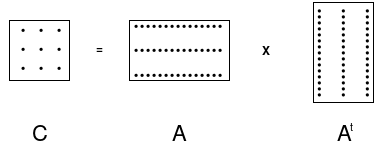
\includegraphics[scale=0.55]{immagini/calcoloSimilarita.png}
        \caption{Calcolo della matrice delle similarità}
        \label{fig:calcoloSimilarità}
     \end{figure}    

Il tesauro è stato generato in maniera automatica, calcolando le co-occorrenze dei termini.
Per fare ciò:
\begin{itemize}
    \item si crea la matrice termini-documenti $A$;
    \item si normalizza la matrice (nel caso specifico si è utilizzato TF-IDF);
    \item si calcola la matrice delle similarità $C = AA^{T}$.
\end{itemize}

Il valore dell'elemento in posizione $C_{i,j}$ della matrice è il valore della similarità tra il termine \textit{i} e il termine \textit{j}.

Si è dovuto quindi determinare una certa soglia oltre la quale i due termini \textit{i} e \textit{j} possono essere considerati simili: la scelta di tale soglia è stata puramente empirica.

%**************************************************************
\section{Latent Semantic Indexing}
\label{comeLSI}
Latent Semantic Indexing (chiamata anche Latent Semantic Analysis) è una tecnica di elaborazione del linguaggio naturale che analizza le relazioni tra un insieme di documenti e di termini che sono contenuti producendo un insieme di concetti legati ai documenti e ai termini. (si veda §\ref{cap:latent-semantic-indexing})

Ai fini del recupero dell'informazione, per semplicità di implementazione, si è deciso di utilizzare la matrice $A_k$: nel caso di un \gls{corpus} grande questo costituirebbe un fattore limitante, ma si è visto che il collo di bottiglia, nella particolare applicazione completamente lato client, è dato invece dal calcolo della decomposizione.

A livello pratico, quindi:
\begin{itemize}
    \item si crea la matrice termini-documenti $A$;
    \item si normalizza la matrice (nel caso specifico si è utilizzato TF-IDF);
    \item si decompone la matrice originale nelle matrici $U$, $S$, $V$ e si calcola $A_k$;
    \item si aggiorna la rappresentazione dei documenti sostituendola con $A_k$;
    \item si aggiorna l'indice inverso (considerando come presente solo i termini oltre una certa soglia).    
\end{itemize}

La scelta del rango(ovvero il numero di concetti) e della soglia oltre la quale considerare un termine è stata, ancora una volta, empirica.

%**************************************************************
\section{Documentazione}
Per produrre la documentazione per lo sviluppatore, si è scelto di utilizzare il tool \gls{jsdoc}, sia per la sua semplicità che per continuità con lunr.js, la libreria principalmente utilizzata. Data la semplicità di utilizzo, non c'è stata necessità di produrre della documentazione per l'utente.             % 
\chapter{Testing}
\label{cap:testing}
\intro{Il capitolo presenta le metriche, come doveva essere costruita la collezione di test e i loro risultati.}\\
\begin{center}
    \begin{figure}
        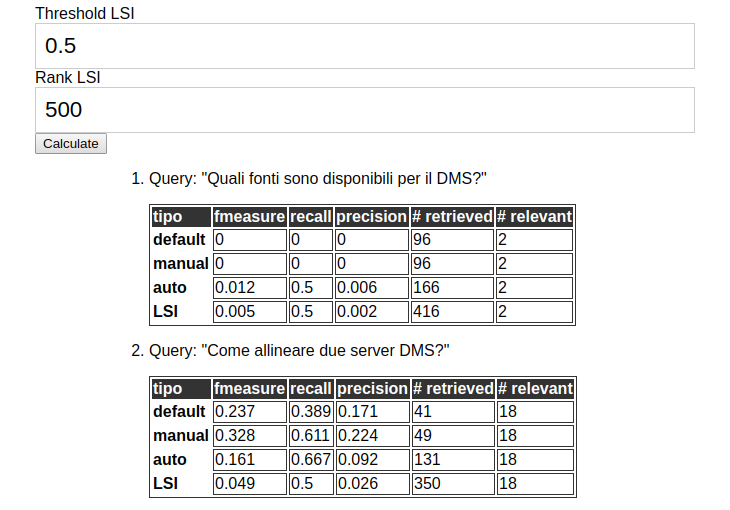
\includegraphics[scale=0.5]{immagini/ir_eval.png}
        \caption{Esempio di risultato dei test
        \label{fig:esecuzioneTest}}
     \end{figure}
\end{center} 
     Parte del lavoro dello stage è stato realizzare una collezione di test che permettessero di valutare la ricerca. Era quindi richiesto, costruire la cosiddetta ground truth, ovvero:
    \begin{itemize}
        \item individuare, per ogni ricerca, quali fossero i documenti pertinenti;
        \item le ricerche dovevano contenere falsi negativi;
        \item le ricerche dovevano essere frasali (e non con un paio di termini).
    \end{itemize}
    Viste le dimensioni del \gls{corpus} e i vincoli precedentemente elencati, sono riuscito ad individuare 20 ricerche con falsi negativi. Un paio di esempi di test è disponibile in §\ref{cap:esempi-test}.

%**************************************************************************
    \section{Metriche}
    Le metriche (f-measure, precision e recall) sono state scelte dall'azienda prima dell'inizio dello stage e sono state presentate in §\ref{sub:metriche-valutazione}.

%************************************************************
\section{Esecuzione dei test}
Per ogni interrogazione, viene generata una tabella(vedi fig. \ref{fig:esecuzioneTest}) contenente:
\begin{itemize}
    \item le misure richieste;
    \item il  numero dei documenti ritornati;
    \item il numero di documenti rilevanti per la ricerca presenti nel \gls{corpus}.
\end{itemize}

I campi del form sono parametri liberi utilizzati nel calcolo della \gls{lsi}: \textit{threshold} è la soglia oltre la quale un termine è considerato presente nel documento, \textit{rank} è il numero dei concetti presenti nel \gls{corpus}. Questo permette di ricalcolare le misure richieste per la soluzione che utilizza l'analisi della semantica latente senza ricalcolare tutto da capo, evitando così di dover rifare calcoli più computazionalmente onerosi (ovvero il calcolo della \gls{svd}).


    \section{Risultati}
    È risultato evidente dai test che la soluzione naive, basata sull'uso di un tesauro manualmente costruito, sia stata quella che ha avuto il miglior risultato: questo probabilmente deriva dal fatto che il \gls{corpus} era piccolo nel complesso e i documenti erano anch'essi piccoli. (i frammenti audio estratti dal servizio di trascrizione) Nella pagina dei risultati dei test è possibile modificare i parametri di soglia e rango della matrice,  senza dover ricalcolare la decomposizione (che è onerosa in termini di tempo).

    \FloatBarrier
%% !TEX encoding = UTF-8
% !TEX TS-program = pdflatex
% !TEX root = ../tesi.tex

%**************************************************************
\chapter{Descrizione dello stage}
\label{cap:descrizione-stage}
%**************************************************************

\intro{Breve introduzione al capitolo}\\

%**************************************************************
\section{Introduzione al progetto}

%**************************************************************
\section{Analisi preventiva dei rischi}

Durante la fase di analisi iniziale sono stati individuati alcuni possibili rischi a cui si potrà andare incontro.
Si è quindi proceduto a elaborare delle possibili soluzioni per far fronte a tali rischi.\\

\begin{risk}{Performance del simulatore hardware}
    \riskdescription{le performance del simulatore hardware e la comunicazione con questo potrebbero risultare lenti o non abbastanza buoni da causare il fallimento dei test}
    \risksolution{coinvolgimento del responsabile a capo del progetto relativo il simulatore hardware}
    \label{risk:hardware-simulator} 
\end{risk}

%**************************************************************
\section{Requisiti e obiettivi}


%**************************************************************
\section{Pianificazione}             % Kick-Off

%% !TEX encoding = UTF-8
% !TEX TS-program = pdflatex
% !TEX root = ../tesi.tex

%**************************************************************
\chapter{Progettazione e codifica}
\label{cap:progettazione-codifica}
%**************************************************************

\intro{Breve introduzione al capitolo}\\

%**************************************************************
\section{Tecnologie e strumenti}
\label{sec:tecnologie-strumenti}

Di seguito viene data una panoramica delle tecnologie e strumenti utilizzati.

\subsection*{Tecnologia 1}
Descrizione Tecnologia 1.

\subsection*{Tecnologia 2}
Descrizione Tecnologia 2

%**************************************************************
\section{Ciclo di vita del software}
\label{sec:ciclo-vita-software}

%**************************************************************
\section{Progettazione}
\label{sec:progettazione}

\subsubsection{Namespace 1} %**************************
Descrizione namespace 1.

\begin{namespacedesc}
    \classdesc{Classe 1}{Descrizione classe 1}
    \classdesc{Classe 2}{Descrizione classe 2}
\end{namespacedesc}


%**************************************************************
\section{Design Pattern utilizzati}

%**************************************************************
\section{Codifica}
             % Product Prototype
%% !TEX encoding = UTF-8
% !TEX TS-program = pdflatex
% !TEX root = ../tesi.tex

%**************************************************************
\chapter{Verifica e validazione}
\label{cap:verifica-validazione}
%**************************************************************             % Product Design Freeze e SOP
% !TEX encoding = UTF-8
% !TEX TS-program = pdflatex
% !TEX root = ../tesi.tex

%**************************************************************
\chapter{Conclusioni}
\label{cap:conclusioni}
%**************************************************************

\section{Risultato ottenuto}
\begin{longtable}{lp{.48\textwidth}p{.15\textwidth}}
    \toprule
        \thcell{Id Requisito} & \thcell{Descrizione} & \thcell{Raggiunto}\\
        \midrule
        \endfirsthead
        % intestazione normale
        \multicolumn{3}{l}{\footnotesize\itshape
        Continua dalla pagina precedente} \\
        \toprule
        \thcell{Id Requisito} & \thcell{Descrizione} & \thcell{Raggiunto}\\
        %\midrule
        \endhead
        % piede normale
        %\midrule
        \multicolumn{3}{r}{\footnotesize\itshape
        Continua nella prossima pagina} \\
        \endfoot
        % piede finale
    \bottomrule
    \caption[Requisiti raggiunti]{Requisiti raggiunti}
    %\multicolumn{3}{r}{\footnotesize\itshape Si conclude dalla pagina precedente} 
    \\
    \endlastfoot
        RF1 & L'utente deve poter effettuare una ricerca all'interno del \gls{corpus} & Sì \\ \addlinespace
        RF2 & Implementazione di una collezione di test per valutare il sistema di ricerca mediante calcolo della precision, recall e f-measure& Sì \\ \addlinespace
        RF3 & Implementazione di una pagina di ricerca dei documenti all'interno del \gls{corpus} che utilizzi un tesauro generato manualmente & Sì\\ \addlinespace
        RF4 & Implementazione di una pagina di ricerca dei documenti all'interno del \gls{corpus} che utilizzi un \gls{autoencoder} & Sì\\ \addlinespace
        RF5 & Implementazione di una pagina di ricerca dei documenti all'interno del \gls{corpus} che utilizzi l'analisi della semantica latente & Sì\\ \addlinespace
        RF6 & Implementazione di una pagina di ricerca dei documenti all'interno del \gls{corpus} che utilizzi un \gls{autoencoder} & No\\ \addlinespace
        RF7 & Implementazione di una pagina di ricerca dei documenti all'interno del \gls{corpus} che utilizzi di un \gls{ensemble} dei metodi (tesauro manuale, tesauro automatico, analisi della semantica latente e \gls{autoencoder}) & No\\ \addlinespace
        RF8 & Implementazione di una pagina di ricerca dei documenti all'interno del \gls{corpus} che utilizzi un tesauro generico (di LibreOffice) & Sì\\ \addlinespace
        RF9 & I risultati delle ricerche devono essere aggregati per ID continui, quindi ordinati in base allo score & Sì \\ \addlinespace
        RF10 & Configurazione dello stemmer italiano & Sì \\ \addlinespace
        RV11 & Il prodotto deve essere eseguibile da browser (su Windows 10, browser Chrome $\geq$ 77.0.3865) & Sì \\ \addlinespace
        RQ12 & Deve essere fornita documentazione in inglese del codice in formato \gls{jsdoc} & Sì \\ \addlinespace
%%%%%% end data
\label{tabella:requisitiCompletati}
\end{longtable}
Non sono riuscito a completare tutti gli obiettivi prefissati all'inizio dello stage,
per le difficoltà emerse e già analizzate in §\ref{sec:problematiche}.
Anche se fossi riuscito ad implementare anche i restanti obiettivi, questo probabilmente
non avrebbe avuto un impatto nel miglioramento del recupero dell'informazione:
come evidenziato anche dal mio tutor aziendale, il \gls{corpus} era insufficiente
per riuscire ad estrarre efficacemente delle informazioni che potessero essere utili 
al fine del reperimento.

Si sarebbe potuto ottenere di più per esempio cercando di espandere il contesto
invece che di estrarre l'informazione dal \gls{corpus}: guardando in letteratura,
infatti, si possono trovare esempi (anche se pochi) che utilizzano le reti di Markov
e un contesto più ampio (Wikipedia in primis come fonte) su \gls{corpus} piccoli. 
Tale approccio però avrebbe richiesto uno sforzo sia dal punto di vista tecnologico (capire
come riadattare la libreria usata per il recupero dell'informazione o cercarne 
un'altra) che dal punto di vista di conoscenze mie (reti di Markov, in particolare),
non compatibile con i tempi dello stage. 

Ritengo sia più quello sono riuscito a ricevere dallo stage che quello che sono riuscito a dare a dare all'azienda: posso dire di portarmi a casa conoscenze in più, mentre l'azienda se non altro ha avuto la conferma che l'approccio naive è quello che ripaga di più (ed eventualmente di indagare verso un approccio probabilistico e non algebrico).

%*************************************************************
\section{Analisi critica del prodotto e del lavoro di stage}
%*************************************************************
\subsection{Conoscenze possedute e acquisite}
All'inizio dello stage, non avevo praticamente mai utilizzato Javascript (purtroppo appena accennato nel corso di tecnologie web e un aspetto secondario nel progetto). Avevo comunque una conoscenza di base di Python per implementare qualche esercizio di competitive programming e del corso di algoritmi e strutture dati e mi ha comunque permesso di provare ad applicare i primi concetti di recupero dell'informazione (p.es. calcolo di tf-idf) e confrontare le prestazioni della soluzione in Javascript con quella in Python.

Da questa esperienza ho imparato
\begin{itemize}
    \item il linguaggio di programmazione Javascript;
    \item delle basi di Node.js;
    \item i fondamenti del recupero dell'informazione;
    \item a utilizzare una libreria di calcolo scientifico in Javascript (LALOLib).
\end{itemize}

Se sono riuscito a reperire in autonomia il materiale necessario (cercando sia tra libri che paper) è anche per l'esperienza fatta durante il corso di studi.


%*************************************************************
\subsection{Utilizzazione del prodotto}
Il prodotto non era pensato per essere immediatamente utilizzabile, non interfacciandosi con quanto di esistente.
Per quanto riguarda la ricerca che fa uso dell'analisi della semantica latente, non è immediatamente utilizzabile in quanto le prestazioni della libreria in Javascript erano insufficienti anche per un \gls{corpus} di piccole dimensioni (circa 75 secondi per decomporre la matrice contro il mezzo secondo scarso di NumPy e i qualche manciata di centesimi di secondo con SciPy): purtroppo non ci sono alternative migliori in Javascript attualmente disponibili. 
Questi calcoli potrebbero essere effettuati lato server, ma comunque rimane una soluzione troppo inefficiente: specialmente se consideriamo che la quantità di testo trascritto è comunque relativamente piccola e corrisponde a circa 4 ore di filmato.

%*************************************************************
\subsection{Valutazione degli strumenti principalmente utilizzati}
\subsubsection{Javascript}
Meno banale di quello che potrebbe sembrare all'inizio: giusto per citare due particolarità, l'ereditarietà prototipale e le immediately invoked function expression. A volte lascia un po' troppe libertà. Mi ha sorpreso non trovare, tra le funzionalità "già incluse" (ovvero senza usare librerie esterne), una coda di priorità.

\subsubsection{lunr.js}
Semplice da usare se si conosce Javascript, ben documentato e lo sviluppo è attivo. Mi ha sorpreso positivamente e di poterlo riutilizzare in futuro. Di negativo c'è che non è ancora compatibile con i moduli di ES6\footnote{\url{https://github.com/olivernn/lunr.js/issues/401}}. 

\subsubsection{LALOLib}
Facile da utilizzare, discreta la documentazione e molto buono il supporto: anche se non troppo efficiente, le alternative non abbondano (se si deve utilizzare Javascript).     
%*************************************************************
\subsection{Possibili estensioni del prodotto}
Le estensioni possibili, più che nelle funzionalità, nell'approccio:
\begin{itemize}
    \item considerare come documenti non i singoli frammenti ma gruppi un po' più grandi di frammenti (bisogna però trovare il trade-off giusto tra numero di documenti e numero dimensione dei documenti singoli);
    \item provare a migliorare espandendo il contesto(p.es. con Wikipedia, come già accennato all'inizio del capitolo).
\end{itemize} 
             % Conclusioni
\appendix                               
% !TEX encoding = UTF-8
% !TEX TS-program = pdflatex
% !TEX root = ../tesi.tex

%**************************************************************
\chapter{Errori di trascrizione}
\label{cap:esempi-errori}
%**************************************************************
Nella generazione della trascrizione dell'audio, inevitabilmente, vengono commessi alcuni errori di trascrizione e alcune cancellazioni. Alcuni errori sono facilmente individuabili in quanto altri e altri no (p.es. CMS al posto di DMS). Ecco alcuni esempi degli errori presenti nel corpus:
\begin{itemize}
    \item \textit{cartelle} diventa \textit{Dell}
    \item \textit{gadget} diventa \textit{viaggio}
    \item \textit{DMS} diventa \textit{DNS, BMS, CMS}
    \item \textit{documenti} diventa \textit{metti, fumetti}
    \item \textit{un attimo} diventa \textit{una chat}
    \item \textit{unità} diventa \textit{vita}
    \item \textit{l’utilità} diventa \textit{tutti dita}
    \item \textit{viaria} diventa \textit{via area}
    \item \textit{filezilla} diventa \textit{un file}
    \item \textit{nostro filesystem fisico} diventa \textit{naso spray System civico}
    \item \textit{configurata} diventa \textit{assicurata}
    \item \textit{appunto} diventa \textit{abita, a}
    \item \textit{il wizard} diventa \textit{Luigia, week}
    \item \textit{acquisizione} diventa \textit{edizione}
    \item \textit{massivi} diventa \textit{Ma Siri}
    \item \textit{Partiamo} diventa \textit{stiamo}
    \item \textit{root} diventa  \textit{Rut}
    \item \textit{ad esempio} diventa \textit{vince}
    \item \textit{log} diventa \textit{zio}
    \item \textit{separazione} diventa \textit{situazione}
    \item \textit{opportuno} diventa \textit{8}
    \item \textit{acquisiamo} diventa \textit{accorge}
    \item \textit{barcode} diventa \textit{Marco}
    \item \textit{sorgente} diventa \textit{so}
    \item \textit{comunque} l’utente diventa \textit{concludente}
    \item \textit{la lettura} diventa \textit{alla Tour}
    \item \textit{sgamato}  diventa \textit{D'Amato}
    \item \textit{consulto il log} diventa \textit{sul tuo blog}
    \item \textit{ha poi} diventa \textit{acqua}
    \item \textit{zmicro} diventa \textit{Desa Minecraft}
    \item \textit{zscanner} diventa \textit{zitta scanner, z-scan}    
    \item \textit{default} diventa \textit{vissuto}
    \item \textit{qui avete} diventa \textit{Piaget}
    \item \textit{produciamo} diventa \textit{provincia}
    \item \textit{nell’XML} diventa \textit{nella ma}
\end{itemize}
%\epigraph{Citazione}{Autore della citazione}



             % Esempi di errori di trascrizione
\chapter{Esempi ground truth}
\label{cap:esempi-test}

\begin{verbatim}
  {
    query: "Come attivare il supporto FTP per DMS?",
    videoIDs: ["353", "354", "355", "356", "357", "358", "359"]
  },
  {
    query: "Come autenticarsi via ftp dopo reboot server java?",
    videoIDs: ["356", "357"]
  },
  {
    query: "Come importare i documenti via ADF?",
    videoIDs: ["172", "173", "174", "175"]
  },
  {
    query: "Dove vengono salvati i miei dati?",
    videoIDs: ["362", "363", "364"]
  }
\end{verbatim}

%**************************************************************
% Materiale finale
%**************************************************************
\backmatter
% !TEX encoding = UTF-8
% !TEX TS-program = pdflatex
% !TEX root = ../tesi.tex

%**************************************************************
% Bibliografia
%**************************************************************

\cleardoublepage
\chapter{Bibliografia}

\nocite{*}
% Stampa i riferimenti bibliografici
\printbibliography[heading=subbibliography,title={Riferimenti bibliografici},type=book]

% Stampa i siti web consultati
\printbibliography[heading=subbibliography,title={Siti web consultati},type=online]



\printglossary[title=Glossario]
\printglossary[type=\acronymtype,title=Acronimi e abbreviazioni]
\end{document}
